\begin{frame}{Instalación de Apache Ofbiz}

	Apache Ofbiz necesita el 'java development kit' (jdk) descargable en la web: \href{http://www.oracle.com/technetwork/java/javase/downloads/jdk8-downloads-2133151.html}{http://www.oracle.com/technetwork/java/javase/downloads/jdk8-downloads-2133151.html}
	
	Después de la instalación del 'jdk' ejecutamos en el directorio principal del programa : ./gradlew cleanAll loadDefault
	
	Es posible que nos encontremos con un error en la variable JAVA\_HOME.
	\begin{figure}[H]
		\centering
		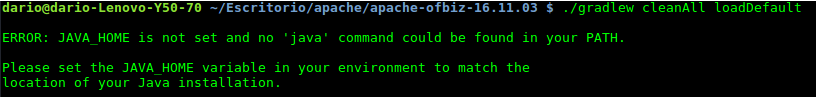
\includegraphics[width=1.0\linewidth]{img/3.png}
	\end{figure}

\end{frame}

\begin{frame}{Solucion del error en la variable JAVA\_HOME}
	Solución:
	\begin{enumerate}
		\item Descargar el archivo .tar.gz de jdk de la página anterior.
		\item Descomprimir y entrar en la carpeta.
		\item Ejecutar JAVA\_HOME=`pwd`, export JAVA\_HOME
		\item volver a la carpeta de Apache Ofbiz y volver a ejecutar ./gradlew cleanAll loadDefault
	\end{enumerate}

\end{frame}

\begin{frame}
Para iniciar el ERP ejecutamos ./gradlew ofbiz.

En la terminal veremos que se muestra una barra de progreso que no avanza del 91\%.
Llegados a este punto Apache ofbiz ya se puede ejecutar.

\begin{figure}[H]
	\centering
	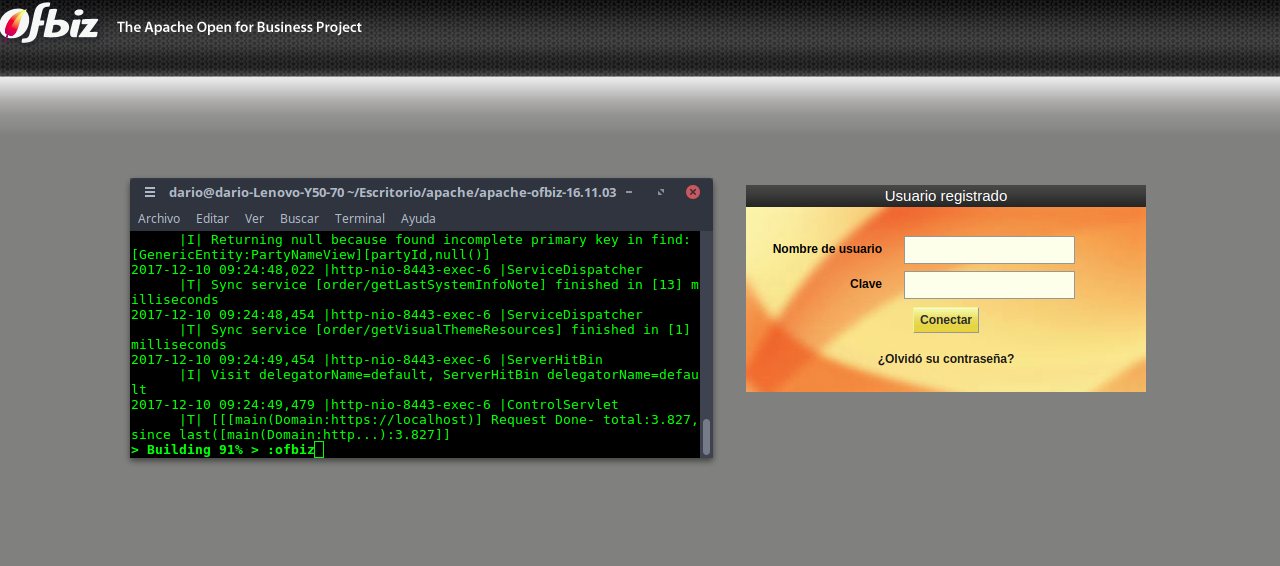
\includegraphics[width=0.65\linewidth]{img/4.png}
\end{figure}

Podemos acceder al ERP desde nuestro navegador:

[Order Back Office](https://localhost:8443/ordermgr)

[Accounting Back Office](https://localhost:8443/accounting)

[Administrator interface](https://localhost:8443/webtools)

La contraseña y el usuario son 'ofbiz' y 'admin' respectivamente, tal y como se explica en el README cuando lo descargamos.
\end{frame}

